%!TEX root = ../dokumentation.tex

\chapter{Implementierung des Graph-Editors}
\label{sec:grapheditor}

Eine der Anforderungen war es, das Modell visuell bearbeiten zu können. Dafür war es notwendig, einen Graph-Editor zu entwickeln. Ein solcher Editor erlaubt es, Knoten hinzuzufügen bzw. zu entfernen und sie miteinander zu verbinden. Der Editor wurde als separate Bibliothek unter dem Namen \textit{BaklavaJS} entwickelt und ist somit auch für andere Projekte verwendbar.

Der Graph besteht aus Knoten und Kanten. Ein Knoten ist dabei wie eine mathematische Funktion: Er führt einen Algorithmus auf die Eingangsdaten aus und gibt die erzeugten Ausgangsdaten aus. Im Gegensatz zu einem \enquote{herkömmlichen} Graphen kann ein Knoten mehrere Kanten zu einem anderen Knoten haben.

Visuell wird ein Knoten in BaklavaJS folgendermaßen dargestellt:

\begin{figure}[H]
    \centering
    \includegraphics[width=.5\textwidth]{node_parts.png}
    \caption{Aufbau eines Knotens in BaklavaJS}
    \label{fig:nodeparts}
\end{figure}

Jeder Knoten besteht aus drei Teilen:
\begin{itemize}
    \item \textbf{Input Interfaces}: Die Eingangsschnittstellen eines Knotens werden benutzt, um Daten von anderen Knoten an diesen Knoten zu transferieren. Ist kein anderer Knoten verbunden, kann der Wert mittels eines Steuerelements auch direkt am Knoten eingestellt werden.
    \item \textbf{Options}: Hier können Werte eingestellt werden, die der Knoten für die Berechnung braucht, die aber beispielsweise zu komplex sind, um als Daten von anderen Knoten über Eingangsschnittstellen zu kommen.
    \item \textbf{Output Interfaces}: Die Ausgangsschnittstellen stellen das Ergebnis bereit, damit es von anderen Knoten benutzt werden kann.
\end{itemize}

\section{Ausführungsreihenfolge des Graphen}

\begin{figure}[H]
    \centering
    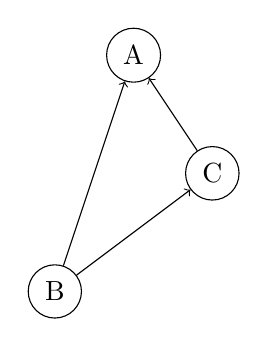
\begin{tikzpicture}
        \node[shape=circle,draw=black] (A) at (0,0) {A};
        \node[shape=circle,draw=black] (B) at (-1,-3) {B};
        \node[shape=circle,draw=black] (C) at (1,-1.5) {C};
        \path[->](B) edge node[left] {} (A);
        \path[->](B) edge node[left] {} (C);
        \path[->](C) edge node[left] {} (A);
    \end{tikzpicture}
    \caption{Beispielgraph}
    \label{fig:nodeExecutionOrder1}
\end{figure}

In Abbildung \ref{fig:nodeExecutionOrder1} ist ein Beispielgraph mit Knoten und Kanten zu sehen. Der Graph kann als Abhängigkeitsgraph interpretiert werden: Um den Knoten $A$ auszuführen, müssen vorher die Knoten $B$ und $C$ ausgeführt werden, damit die Ergebnisse dieser Knoten verfügbar sind. Auch muss der Knoten $B$ vor dem Knoten $C$ ausgeführt werden. $B$ hat keine Abhängigkeiten. Somit ergibt sich als Ausführungsreihenfolge $B \rightarrow C \rightarrow A$.

Die Ausführungsreihenfolge der Knoten muss folgende Bedingungen erfüllen:
\begin{itemize}
    \item Jeder Knoten wird genau einmal ausgeführt
    \item Ein Knoten kann erst ausgeführt werden, wenn alle Knoten, die Kanten zu ihm haben, ausgeführt wurden
\end{itemize}

\todo{Topological Sorting}

Topologische Sortierung kann nur auf azyklischen, gerichteten Graphen durchgeführt werden. Anhand des folgenden, zyklischen Graphen ist das leicht erkennbar:
\begin{figure}[H]
    \centering
    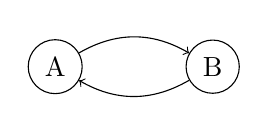
\begin{tikzpicture}
        \node[shape=circle,draw=black] (A) at (-1,0) {A};
        \node[shape=circle,draw=black] (B) at (1,0) {B};
        \path[->](A) edge[bend left] node[left] {} (B);
        \path[->](B) edge[bend left] node[left] {} (A);
    \end{tikzpicture}
    \caption{Zyklischer Graph}
    \label{fig:cyclicGraph}
\end{figure}
Knoten $B$ hat Knoten $A$ als Abhängigkeit. Somit muss Knoten $B$ vor Knoten $A$ ausgeführt werden. Allerdings hat $B$ den Knoten $A$ als Abhängigkeit. Es müsste somit der jeweils andere Knoten zuerst berechnet werden, was nicht möglich ist. Aus diesem Grund darf der Graph keine Zyklen enthalten.

Es gibt bereits Algorithmen, die eine topologische Sortierung eines Graphen ermöglichen. Ein Beispiel davon ist Kahns Algorithmus \cite{Kahn:1962}. Jedoch war in einem Vorgängerprojekt dieser Arbeit bereits ein Algorithmus zur Errechnung einer topologischen Sortierung implementiert und getestet worden. Um keine neuen Fehler in die Applikation zu bringen, wurde der selbst entwickelte und ausführlich getestete Algorithmus in dieser Arbeit verwendet.

Der Algorithmus setzt sich aus drei Teilen zusammen:
\begin{enumerate}
    \item Adjazenzliste für alle Knoten erstellen
    \item Baum aufbauen mit Zykluserkennung
    \item Breitensuche, um die Ausführungsreihenfolge zu bestimmen 
\end{enumerate}

Zuerst wird aus dem Modell für jeden Knoten eine Adjazenzliste erstellt. Eine Adjazenzliste ist eine Liste, die für den Knoten $k_0$ alle Knoten $k$ aus der Knotenmenge $K$ enthält, die eine Verbindung $V(k, k_0)$ zum Knoten $k_0$ haben.

Formal ist die Adjazenzliste für $k_0$ folgendermaßen definiert: $\{ k \in K : V(k, k_0) \}$

Der zweite Schritt des Algorithmus baut einen Baum aus der Adjazenzliste auf. Dies wird durch die \texttt{findChildren}-Funktion erreicht. Die Funktion gibt einen neuen Baumknoten zurück, welcher den aktuellen Knoten $c$ sowie die Adjazenzliste von $c$ als Parameter übergebenen Knoten zurück.

Die 

Die Wurzel des Baums wird durch die Menge aller Knoten dargestellt, welche keine Ausgangsschnittstellen haben.

\begin{algorithm}[H]
    \caption{Baum aufbauen mit Zykluserkennung}
    \begin{algorithmic}[1]
        \Function{findDescendants}{treeNode, ancestors}
            \ForAll{$c$ in $treeNode.children$}
                \If{$c$ in $ancestors$}
                    \State Cycle detected
                \EndIf
                \State $ancestors.push(c)$
                \State $c.children = findChildren(c)$
                \State \Call{findDescendants}{c, ancestors}
                \State $ancestors.pop()$
            \EndFor
        \EndFunction
    \end{algorithmic}
\end{algorithm}

\begin{algorithm}[H]
    \caption{Breitensuche um die Ausführungsreihenfolge zu bestimmen}
    \begin{algorithmic}[1]
        \State $queue \gets \textbf{new} \ Queue()$
        \State $stack \gets \textbf{new} \ Stack()$
        \State $queue.push(root)$
        \While{\textbf{not} $queue.isEmpty()$}
            \State $current \gets queue.dequeue()$
            \ForAll{$c$ in $current.children$}
                \State $stack.push(c)$
                \State $queue.enqueue(c)$
            \EndFor
        \EndWhile
        \State $calculationOrder \gets \textbf{new} \ List()$
        \While{\textbf{not} $stack.isEmpty()$}
            \State $current \gets stack.pop()$
            \If{\textbf{not} $calculationOrder.contains(current)$}
                \State $calculationOrder.append(current)$
            \EndIf
        \EndWhile
    \end{algorithmic}
\end{algorithm}

\section{Grafische Umsetzung}

Die gesamte Visualisierung des Editors wurde mit VueJS umgesetzt. VueJS ist ein JavaScript Framework zum Erstellen von Browser-Frontends. Ein wichtiges Konzept in Vue sind \textit{Komponenten}. Komponenten sind kleine, eigenständige und wiederverwendbare UI-Elemente \cite{vue:components}.

In Anlehnung an das Model-View-Viewmodel-Pattern ist Vue \textit{reaktiv} gestaltet und bietet Datenbindung \cite{vue:instance}. Reaktiv bedeutet, dass Daten im sogenannten \textit{ViewModel} geändert werden können und diese Änderungen direkt in der \textit{View} angezeigt werden.

\begin{figure}[H]
    \centering
    \includegraphics[width=0.8\textwidth]{vue_reactivity.png}
    \caption{Reaktivität in VueJS \cite{vue:reactivity}}
    \label{fig:vuereactivity}
\end{figure}

Die Daten im magentafarbenen Kreis sind die Daten im ViewModel. Werden diese geändert, wird der dazugehörige \textit{Setter} aufgerufen, welcher dafür sorgt, dass die Komponente neu gerendert wird. Beim Rendern werden die neuen Daten übernommen und somit dem Nutzer angezeigt.

\todo{Beispiel einer einfachen Datenbindung}

Durch den komponentenbasierten Ansatz bietet Vue viele praktische Hilfsfunktionen wie etwa bedingtes Anzeigen von Komponenten oder auch das Rendern von Komponenten anhand einer Liste.

\begin{lstlisting}[caption=Rendern von Listen in Vue, label=lst:v-for,language=HTML]
<ul>
    <li v-for="x in array" :key="x">{{ x }}</li>
</ul>
\end{lstlisting}

Wenn es im zugehörigen ViewModel des Codebeispiels \ref{lst:v-for} die Eigenschaft \texttt{array} gibt, wird für jedes Item in der Liste ein neues \texttt{<li>}-Tag im \ac{DOM} erstellt. Für \texttt{array = [1, 2, 3]} würde der Nutzer die folgende Ansicht erhalten:
\begin{itemize}
    \item 1
    \item 2
    \item 3
\end{itemize}

Das gleiche Prinzip wird beim Rendern von Knoten und Kanten verwendet. \todo{sdf}

Diese Art der Wiederverwendbarkeit ist essentiell, um die Knoten und Kanten zu zeichnen. Besonders hilfreich ist hierbei die \texttt{v-for}-Direktive. Sie erlaubt es, eine Liste von Komponenten zu rendern. Dabei werden Änderungen in der Liste über Datenbindung direkt in der UI übernommen. \todo{Mehr Erklärung}



\begin{itemize}
    \item Erklärung VueJS
    \item Wie werden die Kanten gezeichnet?
    \item Wie werden NodeOptions gezeichnet?
    \item Wie wird Zoom / Panning umgesetzt?
\end{itemize}

\section{Plugin-System und Event-System}

\section{Modulares Paketsystem}

\todo{Warum Pakete? Modular = nur das, was man braucht}

Durch das Paketsystem ist BaklavaJS modular aufgebaut und in verschiedene Pakete unterteilt. So wird zum Beispiel für ein Server-Backend keine Visualisierung des Editors benötigt. Aus diesem Grund müssen die Visualisierungs-Plugins nicht installiert werden.

Folgende Pakete sind zum aktuellen Zeitpunkt (Mai 2019) verfügbar:

\begin{itemize}
    \item \textbf{Core}: Dieses Paket enthält alle notwendigen Klassen und Funktionen, um Knoten hinzuzufügen \todo{More}
    \item \textbf{Engine}: Erlaubt es, die Knoten in dem Graphen auszuführen und sorgt dafür, dass Daten über die Kanten übertragen werden
    \item \textbf{Interface-Types}: Fügt Typen zu Knoten-Schnittstellen hinzu. Standardmäßig können nur zwei Schnittstellen mit gleichem Typ miteinander verbunden werden. Es ist aber möglich, Ausnahmen anzugeben, sodass auch Schnittstellen unterschiedlichen Typs miteinander verbunden werden können. Dabei kann auch eine Konvertierungsfunktion mit angegeben werden. So kann zum Beispiel eine Number-Schnittstelle mit einer String-Schnittstelle verbunden werden. Die Konvertierungsfunktion wandelt dabei die Number in einen String um. 
    \item \textbf{Vue-Renderer}: Der Renderer bietet eine Oberfläche für den Editor, welcher im Core implementiert ist.
    \item \textbf{Vue-Options}: Das Vue-Options-Plugin fügt vorgefertigte Knoten-Optionen zum Renderer hinzu.
\end{itemize}